\documentclass[a4paper, 12pt]{article}
\usepackage[includefoot]{geometry} % for typesetting geometry

% LANGUAGE %
%-========-%
\usepackage{luavlna} % for auto non-breaking spaces
\AtBeginDocument{\singlechars{czech}{AaIiVvOoUuSsZzKk}} % chars not to break on

\usepackage[czech]{babel} % czech language localization


% TOC AND LOF %
%-===========-%
\usepackage[titles]{tocloft} % controlling lof and lot
\usepackage[nottoc]{tocbibind} % remove reference to toc from toc

% remove titles from lof and lot, since they are grouped into one section
\makeatletter
\renewcommand\listoffigures{%
    \@mkboth{\MakeUppercase\listfigurename}%
        {\MakeUppercase\listfigurename}%
    \@starttoc{lof}%
}
\renewcommand\listoftables{%
    \@mkboth{\MakeUppercase\listtablename}%
        {\MakeUppercase\listtablename}%
    \@starttoc{lot}%
}
\makeatother

\setlength{\cftfigindent}{0pt} % remove lof indentation
\setlength{\cfttabindent}{0pt} % remove lot indentation

\usepackage{setspace} % for making a more concise toc


% CODE %
%-====-%
\usepackage{minted} % highlight code with Pygments


% GRAPHICS %
%-========-%
\usepackage{graphicx}     % graphics package
\graphicspath{ {./img/} } % path to images

\usepackage{float} % floats in correct position (the [H] option)

\usepackage{subcaption} % for subfigures

\setlength{\fboxsep}{0pt}    % image border separation
\setlength{\fboxrule}{0.5pt} % image border thickness


% TITLE FORMATTING %
%-================-%
\usepackage{titlesec}

% titles have sizes 18pt, 16pt and 14pt, respectively
% the space between the number and the text of the title is 1em
\titleformat{\section}{\bfseries\scshape\fontsize{18pt}{21.6}\selectfont}{\thesection}{1em}{}
\titleformat{\subsection}{\bfseries\fontsize{16pt}{19.2}\selectfont}{\thesubsection}{1em}{}
\titleformat{\subsubsection}{\bfseries\fontsize{14pt}{16.8}\selectfont}{\thesubsubsection}{1em}{}

\titlespacing{\section}      {0pt}{0pt}{6pt} % 18pt (12pt from parskip + 6pt)
\titlespacing{\subsection}   {0pt}{0pt}{4pt} % 16pt (12pt from parskip + 4pt)
\titlespacing{\subsubsection}{0pt}{0pt}{2pt} % 14pt (12pt from parskip + 2pt)


% CROSS-REFERENCES %
%-================-%
\usepackage[hyphens,spaces,obeyspaces]{url} % for formatting urls
\usepackage[hidelinks,unicode]{hyperref} % interactive references

\newcommand*{\fullref}[1]{\hyperref[{#1}]{\ref*{#1}~--~\nameref*{#1}}} % reference number + name


% GRAPHS, CHARTS %
%-==============-%
\usepackage{pgf-pie} % pie charts

% change pie chart number separator from dot to comma
\usepackage{siunitx}
\sisetup{
  output-decimal-marker={,},
  group-separator={\,},
}
\def\ScanPercentage#1\afternumber{\SI{#1}{\percent}}

\usepackage{pgfplots} % bar charts


% BIBLIOGRAPHY %
%-============-%
\usepackage[backend=biber,
            style=iso-numeric, % citations are in style [1], [2]...
            sortlocale=cs_CZ,
            autolang=other,
            bibencoding=UTF8]{biblatex} % use BibLaTeX for references

\addbibresource{soc.bib} % location of the references file

\renewcommand*{\finentrypunct}{} % don't end references with a dot
\renewcommand{\multinamedelim}{\addcomma\space} % use comma as name delimeter
\renewcommand{\finalnamedelim}{\addspace a \space} % "a" between the last 2 names
\renewbibmacro{in:}{} % don't use In: in references
\DeclareFieldFormat{labelnumberwidth}{[#1]} % wrap reference numbers in square brackets


% TABLES          %
% requires: float %
%-===============-%
\usepackage{booktabs} % table formatting

\usepackage{multirow}            % for creating multirow tables
\setlength\heavyrulewidth{0.2ex} % increase top and bottom rule thicknesses

% fixes the issue with babel and multirow: https://tex.stackexchange.com/questions/111999/slovak-and-czech-babel-gives-problems-with-cmidrule-and-cline
\usepackage{etoolbox}
\preto\tabular{\shorthandoff{-}}

 % fixes figure spacing
 % the -8pt should be the default \belowcaptionskip, which doesn't work here for some reason
\BeforeBeginEnvironment{figure}{\vspace{0.5\parskip}}
\AfterEndEnvironment{figure}{\vspace{-0.5\parskip}\vspace{-8pt}}

 % fixes table spacing
\AfterEndEnvironment{table}{\vspace{-\parskip}}

\newcommand{\ra}[1]{\renewcommand{\arraystretch}{#1}} % table row stretching


% MATH %
%-====-%
\usepackage{amsmath, amstext} % for typesetting math
\DeclareMathSymbol{.}{\mathord}{letters}{"3B} % change dot in math to a comma


% CAPTIONS %
%-========-%
\usepackage[font=footnotesize,       % 10pt captions
            justification=centering, % center the captions
            figurename=Obr.,         % picture captions are "Obr."
            tablename=Tab.]{caption} % table captions are "Tab."


% LISTS %
%-=====-%
\usepackage{enumitem} % lists


% DATETIME %
%-========-%
\usepackage[dmyyyy]{datetime}     % dmyyyy datetimes
\renewcommand{\dateseparator}{. } % changes datetime separator


% FONT AND ENCODING %
%-=================-%
\usepackage[T1]{fontenc} % font encoding
\usepackage{fontspec}    % font selector

\setmainfont{CMU Serif}   % font supporting bold smallcaps

\usepackage{fontawesome5} % use FontAwesome 5 for icons


% ACRONYMS %
%-========-%
\usepackage[acronym,                  % use acronyms
            nopostdot,                % no dot at end of 2nd column
            numberedsection,          % number glossary
            nogroupskip,              % no grouping by same letter
            nonumberlist]{glossaries} % no page numbers

\renewcommand{\acrfullformat}[2]{#2\space(#1)} % long (short) to short (long)

\setglossarystyle{alttree} % set style of glossary

% make glossary title spacing be the same as regular title
\renewcommand{\glossarypreamble}{\vspace*{-\baselineskip}\vspace*{-\parskip}}

\makeglossaries

\newacronym{frc}{FRC}{First Robotics Competition}
\newacronym{ftc}{FTC}{First Technical Challenge}
\newacronym{fll}{FLL}{First Lego League}
\newacronym{pdf}{PDF}{Portable Document Format}
\newacronym{html}{HTML}{Hypertext Mark-up Language}
\newacronym{cern}{CERN}{Evropská organizace pro jaderný výzkum}
\newacronym{http}{HTTP}{Hypertext Transfer Protocol}
\newacronym{css}{CSS}{Cascading Style Sheets}
\newacronym{sass}{SASS}{Syntactically Awesome Style Sheets}
\newacronym{cvs}{CVS}{Concurrent Versions System}
\newacronym{cad}{CAD}{Computer-Aided Design}
\newacronym{ftp}{FTP}{File Transfer Protocol}
\newacronym{aes}{AES}{Advanced Encryption Standard}
\newacronym{api}{API}{Application Programming Interface}
\newacronym{si}{SI}{Mezinárodní systém jednotek}
\newacronym{ip}{IP}{Internet Protocol}
\newacronym{png}{PNG}{Portable Network Graphics}
\newacronym{wysiwyg}{WYSIWYG}{What You See Is What You Get}
\newacronym{php}{PHP}{Hypertext Preprocessor}
\newacronym{epub}{EPUB}{Electronic Publication}
\newacronym{mobi}{MOBI}{Mobipocket E-book}
\newacronym{mit}{MIT}{Massachusetts Institute of Technology}
\newacronym{it}{IT}{Information Technology}
\newacronym{www}{WWW}{World Wide Web}
\newacronym{sgml}{SGML}{Standard Generalized Mark-up Language}
\newacronym{https}{HTTPS}{Hypertext Transfer Protocol Secure}
\newacronym{dvi}{DVI}{DeVice-Independent}
\newacronym{ps}{PS}{PostScript}
\newacronym{doc}{DOC}{Microsof Word document}
\newacronym{docx}{DOCX}{Microsoft Word Open XML document}
\newacronym{step}{STEP}{Standard for Exchange of Product model data}

\glsaddall % add all acronyms

% For setting the list of acronyms alignment (note the two extra G's). I didn't
% find a better way to increase the spacing between the acronym and its
% description in the "Seznam zkratek" section, since \glsfindwidesttoplevelname
% only inserts one space.
\glssetwidest{WYSIWYGGG}


% PARAGRAPH FORMATTING %
%-====================-%
\setlength\parindent{0pt} % 0pt paragraph indentation
\setlength\parskip{12pt}  % 12pt paragraph spacing

\renewcommand{\baselinestretch}{1.15} % baseline stretch is 1.15


% OTHER %
%-=====-%
\widowpenalty10000 % prevent widows
\clubpenalty10000  % prevent widows

\pagenumbering{gobble} % suppress page numbering

% define KaTeX logo
\makeatletter
\DeclareRobustCommand{\KaTeX}{%
  K\kern -.19em
  {\sbox \z@ T\vbox to\ht \z@ {\hbox{%
  \check@mathfonts
  \fontsize\sf@size\z@
  \selectfont A}%
  \vss}%
}\kern -.15em
\TeX}
\makeatother

%%%%%%%%%%%%%%%%%%%%%%%%%%%%%%% D O C U M E N T %%%%%%%%%%%%%%%%%%%%%%%%%%%%%%%

\begin{document}
  \sloppy % fixes some lines going to the margins


  % first page's geometry is different
  \newgeometry{top=2.5cm, left=2.5cm, right=2.5cm, bottom=2.5cm}

  \bfseries

  \begin{center}
    {\fontsize{18}{21.6} \selectfont STŘEDOŠKOLSKÁ ODBORNÁ ČINNOST}\\%
    \vspace*{\baselineskip}
    {\fontsize{14}{16.8} \selectfont Obor č. 18: Informatika}\\%

    \topskip0pt
    \vspace{16em}
    {\fontsize{20}{24} \selectfont Robotika Jednoduše}%
    \vspace*{\fill}
  \end{center}

  \fontsize{16}{19.2} \selectfont
  Tomáš Sláma\\
  Liberecký Kraj
  \hfill
  Turnov 2019

  % the geometry for the rest of the document
  \newgeometry{top=2.5cm, left=3.5cm, right=1.5cm, bottom=2.5cm}

  \newpage
  \begin{center}
    {\fontsize{18}{21.6} \selectfont STŘEDOŠKOLSKÁ ODBORNÁ ČINNOST}\\%
    \vspace*{\baselineskip}
    {\fontsize{14}{16.8} \selectfont Obor č. 18: Informatika}\\%

    \topskip0pt
    \vspace{10em}
    \fontsize{20}{24} \selectfont
    Robotika Jednoduše%

    Robotics Simplified%
    \vspace*{\fill}
  \end{center}

  \normalfont
  \fontsize{16}{19.6} \selectfont

  \textbf{Autoři:} Tomáš Sláma\\
  \textbf{Škola:} Gymnázium, Turnov, Jana Palacha 804, příspěvková \\ organizace, 511 21 Turnov \\
  \textbf{Kraj:} Liberecký kraj \\
  \textbf{Konzultant:} Ing. Daniel Kajzr

  \vspace{\baselineskip}

  \fontsize{12}{14.4} \selectfont
  Turnov 2019

  \vspace{4em}

  \newpage

  \section*{\normalfont\textbf{Prohlášení}}
  Prohlašuji, že jsem svou práci SOČ vypracoval/a samostatně a použil/a jsem pouze prameny a literaturu uvedené v seznamu bibliografických záznamů.

  Prohlašuji, že tištěná verze a elektronická verze soutěžní práce SOČ jsou shodné.

  Nemám závažný důvod proti zpřístupňování této práce v souladu se zákonem č.~121/2000 Sb., o právu autorském, o právech souvisejících s právem autorským a o změně některých zákonů (autorský zákon) ve znění pozdějších předpisů.

  \qquad

  V Turnově dne \today \, ..................................................\\%
  \makebox[\linewidth]{Tomáš Sláma}%

  \newpage

  \section*{\normalfont\textbf{Poděkování}}
  V první řadě bych rád poděkoval své rodině a přátelům za neustálou podporu a pozitivitu při tvorbě projektu. Za konzultace o obsahu, struktuře a v projektu použitých technologiích děkuji Ing. Danielovi Kajzrovi, Mgr. Lukáši Pitoňákovi a Mgr. Tomáši Novotnému. Také děkuji Kateřině Sulkové za rady ke psaní samotné SOČ práce a na závěr všem návštěvníkům projektu, kteří svou přítomností a zpětnou vazbou pomáhají v jeho rozvoji.

  \newpage

  \section*{\normalfont\textbf{Anotace}}
  Tato práce popisuje obsah a proces tvorby webové stránky \url{robotics-simplified.com}. Stránka zpracovává témata z oboru robotiky formou pochopitelnou i naprostým začátečníkem. Je poháněna generátorem statických stránek Jekyll, který doplňují JavaSriptové knihovny pro vykreslování matematických rovnic, analýzy návštěvnosti a interaktivní vizualizaci probíraných konceptů. Python skripty automatizují kompresi obrázků, generování souboru sitemap, nahrání obsahu na hosting přes \acrshort{ftp} a převod stránky do knižní podoby pro offline čtení.

  \section*{\normalfont\textbf{Klíčová slova}}
  robotika; webová stránka; vzdělávání

  \section*{\normalfont\textbf{Annotation}}
  This paper describes the contents and the process of creating the \url{robotics-simplified.com} website. The site covers topics in the field of robotics in a beginner-friendly way. It is powered by the static site generator Jekyll, and is suplemented by JavaScript libraries for rendering mathematical equations, analyzing the website traffic and creating interactive visualizations of the discussed concepts. Python scripts fully automate image compression, sitemap file generation, content upload via \acrshort{ftp} and conversion to a book version for offline reading.

  \section*{\normalfont\textbf{Keywords}}
  robotics; website; education

  \newpage

  % resume page numbering
  \newcounter{savepage}
  \setcounter{savepage}{\value{page}}%
  \pagenumbering{arabic}
  \setcounter{page}{\numexpr\value{savepage}-1}%

  % Makes the spacing between toc heading and the contents the same as other
  % section and also makes the item spacing smaller
  \addtocontents{toc}{\vspace{-\cftaftertoctitleskip}\protect\setstretch{0.1}}

  % genereate toc
  \tableofcontents

  \newpage

  % create list of acronyms
  \printglossary[type=\acronymtype, title=Seznam zkratek]

  \newpage

  \section{Úvod}
  V dnešním světě plném technologií se robotika rozvíjí stále rapidnějším tempem. Roboti jsou díky nadaným programátorům a inženýrům rychlejší, obratnější a chytřejší než kdy jindy a uplatnění nalézají v nesčetném množství oborů. Jen za rok 2018 se prodej industriálních robotů zvýšil o 30 \%~\cite{industrial-robot-growth} a nadnárodní korporace jako Amazon jich používají na úkor lidské pracovní síly stále více~\cite{amazon-hiring}. Bez talentovaných lidí by však takový pokrok nebyl možný, proto vzniká řada programů a organizací, které se vzdělávání budoucí generace snaží podporovat.

  Značnou zásluhu má například neziskový program FIRST a jeho soutěže \gls{frc}, \gls{ftc} a \gls{fll}, které z robotiky dělají hru. Týmy tvořeny studenty základních a středních škol mají za úkol během několika týdnů robota od základu navrhnout, postavit a naprogramovat tak, aby plnil úkoly každým rokem se měnící výzvy.

  Začátečníci se zájmem o robotiku se však musí potýkat s problematikou nedostatku studijních materiálů, ať už se jedná o programování robota či o jeho stavbu. Čtení odborných prací není pro každého, zvláště pokud o daném oboru ví málo a hledání přístupnějších zdrojů ne vždy končí úspěchem.

  Stránka \url{robotics-simplified.com}~\cite{robotics-simplified} se snaží tento problém řešit tím, že poskytuje centralizovaný zdroj informací pro nováčky do oboru robotiky. Je strukturována jako série článků, které koncepty intuitivním způsobem vysvětlují. Články obsahují ilustrace a interaktivní vizualizace, a jsou pro zájemce o programování doplněny zdrojovými kódy, které koncepty implementují. Celá stránka je rovněž optimalizovaná pro mobilní zařízení a je dostupná také ve formátu \gls{pdf}, proto připojení k internetu není pro čtení stránky třeba.

  Tato práce se zabývá obsahem a tvorbou výše uvedené webové stránky. Nejprve stanovuje požadavky, které musí výsledný produkt práce splňovat. Poté popisuje programovací jazyky a nástroje, které jsou v projektu využívány a opodstatňuje jejich použití oproti alternativám. Dále rozebírá vývoj, obsah a automatizaci provozu webové stránky a na závěr analyzuje její návštěvnost a získávání zpětné vazby.

  \newpage

  \section{Požadavky na výsledný produkt} \label{sec:Požadavky na výsledný produkt}
  Myšlenka tvorby kvalitních materiálů pro studium robotiky je příliš rozsáhlá na to, aby mohla práce na projektu začít bez větší úvahy~--~bude se jednat o webovou stránku, aplikaci, knihu, či repozitář se zdrojovými kódy?

  Před začátkem je třeba stanovit požadavky, které by výsledný produkt měl splňovat. Podle těch lze způsoby provedení porovnat a použít ten, který se jeví za nejvhodnější.


  \subsection{Otevřenost zdrojového kódu}
  Hlavní požadavek, který by měl produkt splňovat je \emph{otevřenost} (tj. bezplatná dostupnost) zdrojového kódu. Otevřenost výrazně usnadňuje kolaboraci (kdokoliv může navrhnout změnu) a zvyšuje důvěru v daný software (chování programu lze snadno ověřit nahlédnutím do kódu), což jsou pro software zaměřený na vzdělávání kvality žádoucí.

  Příklady populárního otevřeného softwaru využívaného při stavbě tohoto projektu jsou např. Inkscape, Git či Jekyll, které jsou podrobněji rozebírány v kapitole~\ref{sec:Použité nástroje}.


  \subsection{Multiplatformnost}
  Co se dostupnosti týče, důležitým požadavkem je \emph{multiplatformnost}, tj. možnost přístupu k produktu z více než jedné platformy jako stolní počítač, mobil, čtečka elektronických knih, aj. Výsledný produkt musí být multiplatformní zejména kvůli mému osobnímu názoru, že vzdělání by nemělo být omezeno technologickými preferencemi jednotlivce.

  Tato podmínka fakticky znemožňuje tvorbu aplikace, jelikož by jak finanční, tak časové nároky její stavby pro různé operační systémy a zařízení přerostly nad rámec jednotlivce.


  \subsection{Interaktivita}
  Posledním požadavkem je \emph{interaktivita} studijního materiálu, jelikož u technických oborů jako robotika a informatika porozumění nestačí~--~je potřeba si koncepty naživo vyzkoušet. Proto je nutné, aby byl výsledný produkt do určité míry interaktivní a ilustroval probírané koncepty vizualizacemi.

  Kvůli této podmínce nepřipadá v úvahu kniha, jelikož převážná většina populárních formátů pro distribuci knih interaktivitu neumožňuje.


  \section{Použité programovací jazyky} \label{sec:Použité programovací jazyky}
  Programovací jazyk je notace pro psaní programů, které ve své podstatě v slouží k provádění výpočtů. \emph{Syntaxe} jazyka popisuje jeho strukturu~--~jakým způsobem za sebe uspořádat znaky, aby v rámci jazyka tvořily platná spojení, kdežto \emph{sémantika} jazyka popisuje význam těchto platných spojení~\cite{intro-to-programming-languages}.

  Každý programovací jazyk využívá \emph{programovací paradigmata}~--~způsoby, kterými lze přistupovat ke tvorbě programů. Paradigmaty můžeme dělit programovací jazyky do kategorií\footnote{Jeden programovací jazyk může využívat více paradigmat a spadat tak do několika kategorií (viz. jazyky rozebírány v kapitolách~\ref{sec:Python} a~\ref{sec:JavaScript}).} jako např. funkcionální, procedurální, či logické. I přes jejich rozdíly jsou však výpočetně ekvivalentní~--~problém řešitelný v libovolném z nich je nutně řešitelný ve všech.

  Následující kapitola rozebírá v projektu používané programovací jazyky~--~jejich stručnou historii, podstatné principy jejich fungování a jejich roli v projektu. Je nutno dodat, že jsou rozebírány jen jazyky pro funkci projektu nezbytné, jelikož by rozbor všech použitých jazyků byl příliš obsáhlý.


  \subsection{\acrshort{html}} \label{sec:HTML}
  Značkovací jazyk \gls{html} vytvořil Tim Berners-Lee z výzkumného centra \gls{cern} v roce 1989. Hlavní důvod vzniku byla snaha zjednodušit přístup k informacím pomocí virtuálních dokumentů, které by na sebe navzájem odkazovaly a tvořily tím „celosvětovou síť“ sdílených informací \gls{www}. V rámci této snahy Tim rovněž vytvořil protokol \gls{http}, který slouží k přenosu souborů \gls{html} po síti a je k tomuto účelu využíván dodnes~\cite{html-history}.

  Jazyk \gls{html} používá ke strukturování textu tzv. \emph{tagy}~--~slova ohraničená lomítky, která určují význam jimi obklopené části textu. Tento princip značení byl inspirován mezinárodním standardem \gls{sgml}, což bylo s ohledem na dnešní popularitu \gls{html} bezesporu správné rozhodnutí.

  Příkladem \gls{html} je následující ukázka, která se skládá z hlavního nadpisu (\mintinline{html}{<h1>}~--~heading) následovaného paragrafem (\mintinline{html}{<p>}~--~paragraph), ve kterém se dále nachází odkaz na webovou stránku (\mintinline{html}{<a>}~--~anchor):

  \begin{minted}[linenos,breaklines,autogobble]{html}
  <h1>HTML</h1>
  <p>Značkovací jazyk HTML vytvořil Tim Berners-Lee z výzkumného centra <a href="https://home.cern/">CERN</a> v roce 1989.</p>
  \end{minted}

  V \gls{html} psán zdrojový kód převážné většiny webových stránek internetu a tento projekt není výjimkou. Je generován Jekyllem, který je podrobněji rozebírán v kapitole \ref{sec:Jekyll}.


  \subsection{\acrshort{css}} \label{sec:CSS}
  Se stoupající popularitou webu v 90. letech 20. rostla také nespokojenost autorů dokumentů \gls{html} s nedostatky v jeho formátování, jelikož bylo řízeno prohlížeči a nemohlo jimi být žádným způsobem ovlivněno\footnote{To, že v čistém \gls{html} nejde ovlivnit vzhled dokumentu není pravda, ale není to doporučované~--~\gls{html} by mělo být zaměřeno na sémantiku dokumentu, ne na jeho formátování.}. Z tohoto důvodu Håkon Wimu Lie publikoval roku 1994 možné řešení tohoto problému~--~návrh stylopisného jazyka \gls{css}~\cite{css-proposal,css-saga}.

  Při použití \gls{css} je důležitý princip kaskádování (o čemž koneckonců vypovídá zkratka \gls{css})~--~vzhled stránky ovlivňují jak požadavky čtenáře, tak požadavky autora. Samotné kaskádování je kombinace těchto požadavků a v případě vzniku konfliktů (autor požaduje písmo velikosti \texttt{12b}, ale čtenář velikosti \texttt{10b}) jejich rozřešení.

  Příkladem platného souboru \gls{css} je následující ukázka, která upravuje vlastnosti nadpisu \mintinline{html}{<h1>} \gls{html} dokumentu~--~mění jeho barvu textu na zelenou, pozici na střed stránky a velikost na \texttt{18b}:

  \begin{minted}[linenos,breaklines,autogobble]{css}
  h1 {
    color: green;
    font-size: 18pt;
    text-align: center;
  }
  \end{minted}

  V projektu je používán \gls{sass}, který převádí \gls{css} s pokročilejší syntaxí a dodatečnou funkcionalitou do standardního \gls{css}. Díky vyšší míře abstrakce a dodatečným funkcím (jako přidání proměnných, které \gls{css} nepodporuje) lze vzhled stránky upravovat efektivněji.


  \subsection{JavaScript} \label{sec:JavaScript}
  Okolo roku 1995 bylo pro internetový prohlížeč Netscape potřeba vytvořit interpretovaný skriptovací jazyk pro zlepšení interaktivity webových stránek, který by šel vložit přímo do dokumentů \gls{html}. Tímto úkolem byl pověřen Brendan Eich a jelikož bylo z finančních důvodů potřeba práci vykonat rychle, první funkční verze JavaScriptu byla údajně zhotovena za pouhých 10 dní~\cite{the-origin-of-javascript}.

  Na rozdíl od kódu psaném v jazyce \gls{php}, který je vykonáván na straně serveru, je JavaScriptový kód vykonáván na straně uživatele. Kvůli tomu plní na webové stránce funkce, které nevyžadují neustálý kontakt se serverem (jelikož výměna informací tímto způsobem zpravidla není okamžitá) jako kontrola správného vyplnění formuláře, zajištění plynulosti uživatelského prostředí, či tvorba webových her.

  Dnes se jedná o webový standard a dlouhodobě nejpoužívanější programovací jazyk platformy GitHub~\cite{github-statistics}, který zajišťuje vykreslování rovnic, interaktivitu vizualizací, vyhledávání na stránce, aj.


  \subsubsection{p5.js} \label{sec:p5.js}
  p5.js je JavaScriptová knihovna založena na softwaru pro tvorbu interaktivních „skečů“ Processing. Umožňuje vykreslovat tvary a křivky pomocí volání jednoduchých funkcí, proto se jedná o populární volbu pro umělce, učitele, či designéry.


  \subsubsection{\texorpdfstring{\KaTeX}{KaTeX}} \label{sec:KaTeX}
  \KaTeX{} je JavaScriptová knihovna vytvořena pro vzdělávací stránku Khan Academy, která je na stránce používána na renderování matematických rovnic z \LaTeX ové notace (viz. kapitola~\ref{sec:Matematika}).

  Populární alternativou, která byla na stránce dříve používána je populární JavaScriptová knihovna MathJax. Oproti \KaTeX u je však znatelně pomalejší~\cite{katex-mathjax-comparison}, proto již není používána.


  \subsection{Python} \label{sec:Python}
  Python je programovací jazyk vytvořený pro distribuovaný operační systém Amoeba Guidem van Rossumem v 80. letech 20. století. Byl inspirován Guidovou prací na jazyce ABC: „Vzal jsem ingredience z ABC a trochu jsem je promíchal. Python je v mnoha věcech podobný ABC, ale v mnoha také rozdílný“~\cite{making-of-python} (přeloženo z angličtiny).

  Od svého vzniku se Python postupně vyvinul v mocný a frekventovaně používaný programovací jazyk~--~má rozsáhlou standardní knihovnu, podporuje mnoho různých programovacích paradigmat a je třetím nejpoužívanějším programovacím jazykem na platformě GitHub~\cite{github-statistics}, od stavby webových stránek (Django) po knihovny na trénování neuronových sítí (TensorFlow).

  Na stránce zastává funkci skriptovacího jazyka pro automatizaci provozu (viz. kapitola~\ref{sec:Automatizace provozu stránky}). Oproti alternativám jako \gls{php} a Java je na stránce používán převážně díky velkému množství „modulů“ (knihoven), jednoduché syntaxi a mým dlouhodobým zkušenostem s jeho používáním.


  \subsection{Markdown} \label{sec:Markdown}
  Markdown je styl formátování prostého textu, vytvořený v roce 2004 Johnem Gruberem pro autory webových stránek. Je uzpůsobený k jednoduchému čtení, psaní a převodu do pokročilejších značkovacích jazyků jako \gls{html}~\cite{markdown-history}. Jedná se o populární formát zápisu dokumentací projektů, souborů README (čti mě) pro repozitáře stránek jako GitHub a GitLab, či článků některých blogů a osobních stránek.

  Existuje řada „variant“ (z anglického \textit{flavor}) Markdownu jako Kramdown či Redcarpet, které originál rozšiřují o dodatečnou funkcionalitu jako vkládání poznámek pod čarou, podporu úpravy vzhledu stránky pomocí \gls{css} či možnost přidávání rovnic v \LaTeX ové notaci.

  V projektu je v kombinaci s šablonovým jazykem Liquid používán ke psaní článků (viz. kapitola~\ref{sec:Proces tvorby článků}), jelikož právě z nich Jekyll generuje výslednou webovou stránku.


  \subsection{\TeX} \label{sec:TeX}
  \TeX{} je programovací jazyk pro sázení odborné literatury vytvořený Donaldem E. Knuthem v 70. létech 20. století. Počáteční impulz pro vznik byla Knuthova nespokojenost s tiskovou kvalitou vydání jedné z jeho knih, což jej vedlo ke studiu principů sázení, tvorby fontů a později až k vytvoření vlastního sázecího systému \TeX{}~\cite{tex-history}.

  Od \gls{wysiwyg} programů jako Microsoft Word či LibreOffice se \TeX{} liší tím, že autor při psaní nevidí, jak dokument vypadá. Namísto toho pomocí „maker” (souborů instrukcí) definuje, jak by dokument vypadat měl a \TeX{} se o samotné sázení postará. Tento přístup klade větší důraz na obsah~--~autor se formátováním do značné míry nemusí zabývat a může se soustředit na psaní. Další výhoda tohoto přístupu je jednoduchost verzování \TeX ových dokumentů, jelikož jsou psány v prostém textu.

  V projektu je používán \LaTeX{} (viz. kapitola~\ref{sec:Převod webové stránky do PDF}). Jedná se o nadstavbu \TeX u, která díky pokročilejším makrům jako automatické číslování stránek, vkládání referencí, aj. umožňuje pohodlnější tvorbu dokumentů~\cite{getting-started-with-latex}.

  Následující příklad obsahuje část zdrojového kódu \LaTeX ového dokumentu, který definuje nadpis a paragraf, na jehož konec je vložen odkaz na citaci:

  \begin{minted}[linenos,breaklines,autogobble]{latex}
  \subsection{\TeX}
  \TeX{} je programovací jazyk pro sázení odborné literatury vytvořený Donaldem E. Knuthem v 70. létech 20. století~\cite{tex-history}.
  \end{minted}

  K převodu \LaTeX u do formátu \gls{pdf} je v projektu používán český program pdf\TeX, který umožňuje „produkci \gls{pdf} přímo z \TeX ového vstupu bez převodu do přechodných formátů jako \acrshort{dvi} (\acrlong{dvi}~--~původní výstupný formát \TeX u) či \gls{ps}“~\cite{pdftex} (přeloženo z angličtiny).


  \section{Použité nástroje} \label{sec:Použité nástroje}
  Tato kapitola popisuje programy, které jsou používány při vývoji stránky. Hlavní kritérium výběru byla multiplatformnost, jelikož jsou při vývoji aktivně využívány operační systémy Windows a Linux.

  Do této kapitoly nejsou i přes své použití v projektu zahrnuty textový editor Atom a Git klient GitKraken, jelikož pro jeho vývoj nejsou nezbytné.


  \subsection{Git} \label{sec:Git}
  Git je otevřený\footnote{Zdrojový kód Gitu je dostupný na adrese \url{https://github.com/git/git}.} verzovací systém vytvořený Linusem Torvaldsem pro použití na operačním systému Linux. V open-source komunitě se v současné době (31. leden 2019) jedná o nejpoužívanější verzovací systém~\cite{version-control-usage-statistics}, což je jeden z hlavních důvodů pro jeho využití v tomto projektu.

  Verzovací systém umožňuje zaznamenávat změny a jejich důvod/význam na verzované skupině souborů a složek (tzv. repozitáři) a pomáhá tím zamezit ztrátě práce, zjednodušit hledání chyb v kódu a usnadnit spolupráci mezi autory.

  Na rozdíl od centralizovaných verzovacích systémů jako Subversion či \gls{cvs} je Git decentralizovaný~--~místo hlavní úschovny kódu pracuje každý s lokální kopií, která obsahuje úplnou historií projektu. Hlavní výhody tohoto přístupu jsou rychlost práce s repozitářem, možnost pracovat na projektu bez internetového připojení a zamezení ztráty kódu při selhání centrálního serveru~\cite{cvcs-vs-dvcs}.

  Decentralizovanost Gitu však existenci hlavní kopie nezamezuje~--~existuje řada služeb jako GitHub, GitLab či GitBucket, které centrální úschovny pro Gitem verzované projekty (jako tento dokument) hostují a poskytují tím při ztrátě či poškození lokální kopie zálohu.


  \subsection{Jekyll} \label{sec:Jekyll}
  Jekyll je otevřený\footnote{Zdrojový kód Inkscapu je dostupný na adrese \url{https://gitlab.com/inkscape/inkscape}.} generátor statických webových stránek napsaný v jazyce Ruby. Od tradičních přístupů ke stavbě webové stránky využívajících databáze či systém pro správu obsahu se liší tím, že ji generuje pouze z textových souborů udávajících její obsah a vzhled. Výsledný produkt je plně statická stránka, která není napojena na žádný dynamický systém.

  Jelikož je převážná většina souborů projektu prostý text, tak je verzování Jekyllové stránky oproti databázi výrazně jednodušší. Další výhodou je ochrana před potenciálními útoky, jelikož u statických webových stránek není řada frekventovaně využívaných útoků možná~--~hosting si neukládá nic, co by potenciální útočník mohl zneužít.

  Hlavní nevýhodou statických webových stránek je obtížné přidávání dynamicky-se měnícího obsahu jako komentáře či systém přihlašování, ke kterému jsou zpravidla potřeba databáze. Kvůli tomu se nejedná o vhodné technické řešení pro sociální sítě a diskuzní fóra.

  Nejpopulárnější alternativa Jekyllu je Hugo, který byl při vývoji stránky rovněž testován, avšak nakonec byl díky aktivnější komunitě a osobní preferenci zvolen Jekyll.


  \subsection{Inkscape} \label{sec:Inkscape}
  Inkscape je otevřený\footnote{Zdrojový kód Jekyllu je dostupný na adrese \url{https://github.com/jekyll/jekyll}.} multiplatformní software na tvorbu vektorové grafiky. Oproti rastrovým softwarům, které pracují s  pixely obrázku, si vektorové pamatují informace o tom, z jakých tvarů se obrázek skládá, což z nich dělá ideální kandidáty pro tvorbu ilustrací (viz. kapitola~\ref{sec:Ilustrace}).

  Jedná se o populární volbu pro ty, kteří nepoužívají profesionální software jako Adobe Illustrator z důvodu vysoké ceny, uzavřenosti zdrojového kódu či nedostupnosti pro operační systém Linux.


  \subsection{Fusion 360} \label{sec:Fusion 360}
  Ke tvorbě ilustrací k je kromě přístupů rozebíraných v kapitole~\ref{sec:Inkscape} dále používán \gls{cad} software, který slouží ke tvorbě technických nákresů. Na rozdíl od tradičních programů na tvorbu grafiky jsou rozměry tvořených objektů přesně definovány v jednotkách \gls{si}, aby odpovídaly objektům reálného světa.

  Populární \gls{cad} software využíván členy \gls{frc} týmů je Fusion 360 od společnosti Autodesk, převážně kvůli dostupnosti licence (zdarma pro studenty a jejich mentory). Profesionální alternativou je program SolidWorks, který je kvůli své ceně využíván převážně studenty technicky zaměřených škol přes výhodnější školní licenci.

  Fusion 360 je jediný v projektu používaný program, který nefunguje na operačním systému Linux, jelikož s ním mám dlouhodobé zkušenosti. Alternativou je multiplatformní program FreeCAD, se kterým však dostatek zkušeností nemám, proto v projektu používán není.


  \section{Vývoj stránky}
  Po důkladném zvážení výhod a nevýhod přístupů k projektu s požadavky vymezenými kapitolou~\ref{sec:Požadavky na výsledný produkt} se webová stránka jeví jako nejvhodnější výsledný produkt. Může totiž při správném výběru technologií splňovat jak multiplatformnost, tak otevřenost zdrojového kódu.

  Následující kapitoly popisují, jakými způsoby byly různé části stránky (hosting, logo, aj.) řešeny. Za zmínku stojí, že jelikož vývoj těchto částí probíhal paralelně, tak kapitoly nejsou chronologicky řazené.


  \subsection{Technické provedení stránky}
  Pro tvorbu stránky s ohledem na otevřenost jejího zdrojového kódu byl vybrán generátor statických webových stránek Jekyll (viz. kapitola~\ref{sec:Jekyll}). Díky tomu lze kód produktu verzovat a volně sdílet jednodušeji, než kód webové stránky s databází.

  Po zvážení možností zdarma dostupných otevřených šablon pro Jekyll byla zvolena šablona Just the Docs, která díky své optimalizaci pro mobilní zařízení pomáhá s multiplatformností projektu. Další atraktivní vlastnosti této šablony jsou její přehlednost, vestavěná podpora vyhledávání a přizpůsobitelné zvýrazňování syntaxe kódu.


  \subsection{Webhosting a doména} \label{sec:Webhosting a doména}
  Na českém trhu operuje řada firem, které zajišťují jak registraci domény, tak hostování webové stránky. Každá má své výhody a nevýhody, proto je volba provozovatele vysoce individuální a záleží na řadě faktorů.

  Stránka je hostována a doména zprostředkována společností WEDOS Internet a její službou NoLimit, zejména díky mým pozitivním zkušenostem s tímto provozovatelem v rámci minulých projektů a faktem, že ceny a parametry služeb jiných hostingů se od využívané příliš neliší.

  Další možností hostingu je služba GitHub Pages, která umožňuje přes GitHub hostovat stránku generovanou Jekyllem. Hosting i doména by byly zdarma, nebylo by třeba obsah nahrávat přes \acrshort{ftp} a generování by po provedení změny v repozitáři proběhlo automaticky. Tento přístup však neumožňuje využívání Python skriptů, proto není pro účely projektu vhodný.


  \subsection{Design loga}
  Na dobré vizáži každé stránky má značný podíl její logo, které by mělo tematicky odpovídat zaměření stránky bez toho, aby bylo příliš komplikované.

  Hlavní myšlenka za vzhledem loga je spojení výrazů „RO“ a „SI“ (první dvě písmena názvu stránky) do jednoho. Toto spojení výrazy zjednodušuje a tematicky tak odpovídá obsahu webové stránky, která je založena na jednoduchosti. Tvar písmene „O“ je rovněž podobný ozubenému kolu, což do designu loga pro stránku zaměřenou na robotiku elegantně zapadá.

  \begin{figure}[H]%
    \centering

    \subcaptionbox{Počáteční nápad}{
\includegraphics[width=.3\linewidth]{logo1.png}}%
    \hfill
    \subcaptionbox{Přidání ozubeného kola}{
\includegraphics[width=.3\linewidth]{logo2.png}}%
    \hfill
    \subcaptionbox{Konečná podoba}{
\includegraphics[width=.3\linewidth]{logo3.png}}%

    \caption{Design loga stránky}%
    \label{img:Design loga stránky}%
  \end{figure}

  K designu loga byl použit program na úpravu vektorové grafiky Inkscape (viz. kapitola~\ref{sec:Inkscape}).


  \subsection{Verzování zdrojového kódu}
  Stránka je verzována pomocí verzovacího systému Git (viz. kapitola~\ref{sec:Git}). Kód je otevřený a volně dostupný přes GitHub na adrese \url{https://github.com/xiaoxiae/Robotics-Simplified-Website} a rovněž jako příloha této práce (viz. kapitola \ref{sec:Příloha 1: Zdrojový kód webové stránky}).

  Kromě větších binárních souborů jako ilustrace, které se mohou při revizích článků měnit a zbytečně tak zvětšovat velikost repozitáře, jsou verzovány všechny negenerované soubory udávající vzhled a obsah stránky.


  \subsection{Testování výkonu}


  \subsubsection{Doba načtení}
  Doba načtení webové stránky je jedním z hlavních faktorů ovlivňujících její úspěšnost. Přebytečný čas nad optimální dobu (mezi $1.8$ a $2.7$ vteřinami) má negativní vliv na procento konverzí stránky. Při zpoždění o $100$ milisekund nad tuto dobu klesá toto procento pro uživatele osobních počítačů o $7.8$ \%. Konverze dále klesají až o $26.2$ \% při zpoždění v řádu $2$ vteřin~\cite{conversion-rate-statistics}.

  Testování bylo provedeno s pomocí služby \url{https://www.webpagetest.org/}, která analyzuje webové stránky z různých lokací světa (a různých prohlížečů) a poskytuje statistiky o rychlosti načtení, množství načtených dat a mnohém dalším.

  Obrázek~\ref{img:Mapa dob načtení z různých lokací světa} obsahuje informace o době \emph{úplného načtení} (tj. přenesení všech potřebných dat) stránky \url{http://robotics-simplified.com/} z většiny dostupných testovacích lokalit výše uvedené služby ke 13. únoru 2019. Všechna data z testování jsou dostupná jako příloha této práce (viz. kapitola \ref{sec:Příloha 2: Data testování doby načtení}).

  \begin{figure}[H]
    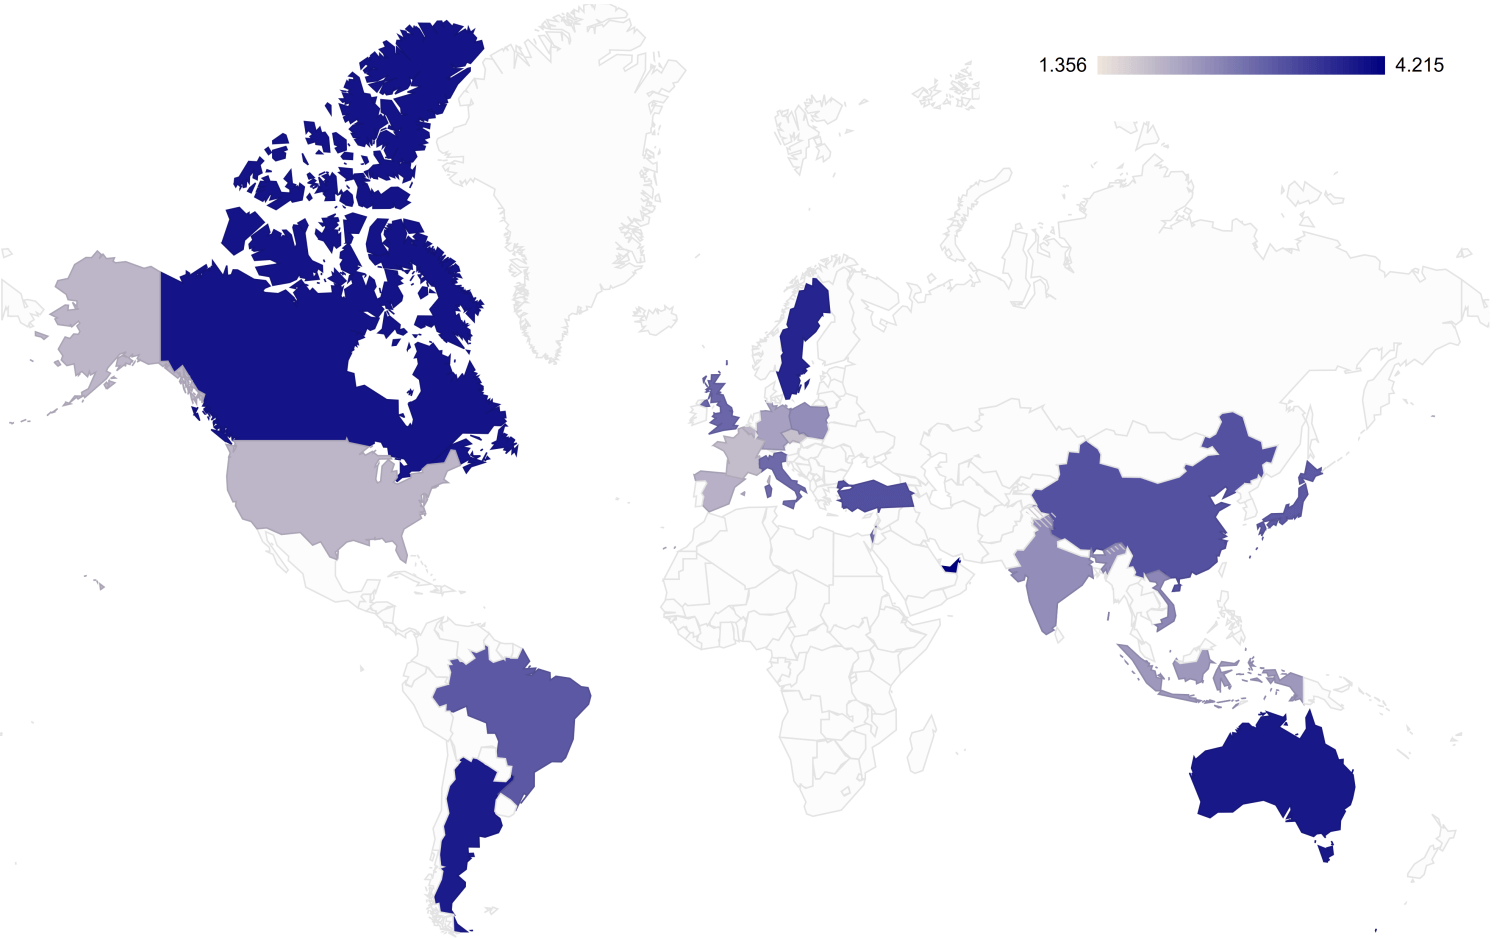
\includegraphics[width=\linewidth]{map.png}
    \caption{Mapa dob načtení z různých míst světa} \label{img:Mapa dob načtení z různých lokací světa}
  \end{figure}

  Z obrázku~\ref{img:Mapa dob načtení z různých lokací světa} je patrné, že doba načtení webové stránky je do značné míry závislá na vzdálenosti od České republiky, ve které je hostována. Tyto hodnoty v testovaných zemích rovněž výrazně nepřevyšují optimální dobu, což je při uvážení ceny webhostingu více než přijatelné.


  \subsubsection{Multiplatformnost}
  Jelikož je výsledný produkt webová stránka, tak další kritický faktor ovlivňující její úspěšnost je správné fungování na různých typech zařízení a prohlížečích.

  Funkčnost různých komponent stránky byla testována na několika z nejpoužívanějších prohlížečů světa~\cite{browser-statistics}: Firefox 65.0.1 (\faIcon{firefox}), Chrome 72.0.3626.105 (\faIcon{chrome}), Internet Explorer 11.590.17134.0 (\faIcon{internet-explorer}), Edge 42.17134.1.0 (\faIcon{edge}), Safari 12.0, 14606.1.36.1.9 (\faIcon{safari}) a Opera 58.0.3135.79 (\faIcon{opera}). Testování se skládalo z načtení stránky na příslušném prohlížeči a kontroly, zda testované komponenty fungují tak, jak by měly.

  Výsledky těchto testů jsou zaneseny do tabulky \ref{tab:Funkčnost stránky na různých platformách}~--~správné fungování je značeno symbolem \faIcon{check}, špatné symbolem \faIcon{times} a nemožnost testování z důvodu nedostupnosti prohlížeče na dané platformně je značeno symbolem \faIcon{minus}.

  \begin{table}[H]
    \caption{Funkčnost stránky na různých platformách}
    \label{tab:Funkčnost stránky na různých platformách}
    \footnotesize
    \centering
    \ra{1.3}
    \begin{tabular}{@{}rccccccccccccc@{}} \toprule
      & \multicolumn{6}{c}{Stolní počítač} & \phantom{abc} & \multicolumn{6}{c}{Mobilní zařízení} \\
        \cmidrule{2-7} \cmidrule{9-14}
       & \faIcon{firefox} & \faIcon{chrome} & \faIcon{internet-explorer} & \faIcon{edge} & \faIcon{safari} & \faIcon{opera}
      && \faIcon{firefox} & \faIcon{chrome} & \faIcon{internet-explorer} & \faIcon{edge} & \faIcon{safari} & \faIcon{opera}\\
        \midrule
      Zobrazení obrázků     & \faIcon{check} & \faIcon{check} & \faIcon{check} & \faIcon{check} & \faIcon{check} & \faIcon{check}
      && \faIcon{check} & \faIcon{check} & \faIcon{minus} & \faIcon{check} & \faIcon{check} & \faIcon{check} \\
      Zobrazení rovnic     & \faIcon{check} & \faIcon{check} & \faIcon{check} & \faIcon{check} & \faIcon{check} & \faIcon{check}
      && \faIcon{check} & \faIcon{check} & \faIcon{minus} & \faIcon{check} & \faIcon{check} & \faIcon{check} \\
      Interaktivita vizualizací & \faIcon{check} & \faIcon{check} & \faIcon{times} & \faIcon{check} & \faIcon{check} & \faIcon{check}
      && \faIcon{check} & \faIcon{check} & \faIcon{minus} & \faIcon{check} & \faIcon{check} & \faIcon{check} \\
      Formátování & \faIcon{check} & \faIcon{check} & \faIcon{check} & \faIcon{check} & \faIcon{check} & \faIcon{check}
      && \faIcon{check} & \faIcon{check} & \faIcon{minus} & \faIcon{check} & \faIcon{check} & \faIcon{check} \\
        \bottomrule
    \end{tabular}
  \end{table}

  Z tabulky \ref{tab:Funkčnost stránky na různých platformách} je patrné, že stránka funguje správně na všech prohlížečích a zařízeních kromě Internetu Explorer, který na mobilu dostupný není a na počítači nenačte vizualizace. S ohledem na procento návštěvníků stránky používajících Internet Explorer (viz. tabulka \ref{tab:Návštěvnost stránky podle prohlížeče}) jsou výsledky velmi uspokojivé.


  \section{Obsah stránky}
  Obsah projektů zaměřených na vzdělání je jejich nejdůležitější čast, jelikož i skvěle vypadající webová stránka s těžce pochopitelnými články svůj účel vzdělávání návštěvníků nesplní.

  Následující kapitola nejprve popisuje cílovou skupinu, pro kterou je obsah stránky tvořen. Poté popisuje proces tvorby článků a jejich dílčích částí. Následně rozebírá strukturu obsahu a na závěr jeho možná uplatnění.


  \subsection{Cílová skupina}
  Při tvorbě studijních materiálů je v první řadě třeba vymezit jeho cílovou skupinu, protože od ní se odvíjí vše ostatní~--~jazyk textu, obtížnost použité matematiky, detail ilustrací, aj. Při výběru musí být brána v potaz především úroveň vzdělávání autora, jelikož středoškolský student experta v oboru mnoho nenaučí.

  Do cílové skupiny proto patří lidé v podobné situaci, ve které jsem byl já na konci roku 2017 krátce po mém vstoupení do \gls{frc} týmu Metal Moose~--~jedinci se zájmem o robotiku, které od studia odrazuje nedostatek intuitivních a lehce pochopitelných materiálů. Kvůli tomu, že jsem až donedávna do této skupiny patřil, dokáži snadněji psát takové články, které bych si při mých začátcích s robotikou přál číst.

  Předešlé znalosti v oblasti robotiky či elektrotechniky pro čtení článků stránky potřebné nejsou, doporučeny jsou pouze základní znalosti programování a středoškolské matematiky (geometrie, algebra).


  \subsection{Proces tvorby článků} \label{sec:Proces tvorby článků}
  Při tvorbě nového článku je nejprve zvoleno téma, které bude článek rozebírat. Vyšší prioritu mají témata, jejichž pochopení pro mě bylo z dostupných internetových zdrojů náročné. Další faktory ovlivňující tento výběr jsou obtížnost zařazení tématu do již vytvořených tématických okruhů a jeho užitečnost v soutěži \gls{frc}.

  Po vybrání tématu článku jsou shromážděny dostupné materiály~--~prezentace, odborné práce, články, aj. Poté jsou seřazeny podle jejich podílu na mém pochopení daného tématu a na stránce následně zmíněny jako dodatečné studijní materiály.

  Hlavní koncepty těchto témat jsou dále implementovány přes online prostředí RobotMesh v jazyce Python na robotovi ze stavebnice VEX EDR, který byl pro tento účel vytvořen. Dva úhly pohledu na jeho konstrukci zachycuje obrázek \ref{img:3D Model robota}, který byl zhotoven v \gls{cad} programu Fusion 360. Zdrojový kód tohoto modelu je dostupný jako příloha této práce (viz. kapitola \ref{sec:STEP model robota}) ve formátu \gls{step}.

  \begin{figure}[H]%
    \centering

    \subcaptionbox{Boční pohled na model robota}{\fbox{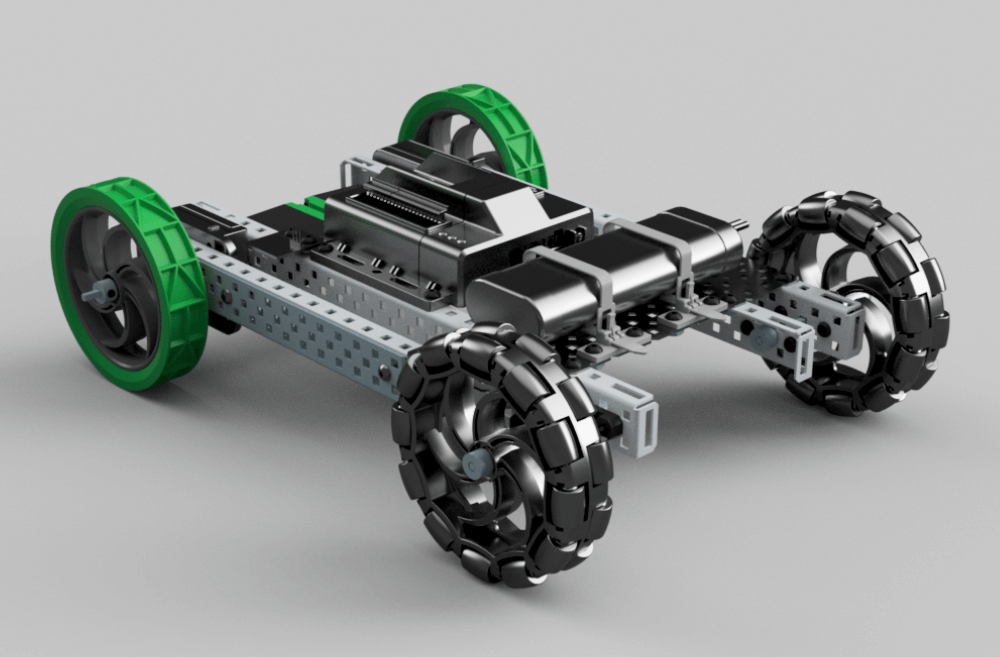
\includegraphics[width=.475\linewidth]{robot1.png}}}%
    \hfill
    \subcaptionbox{Horní pohled na model robota}{\fbox{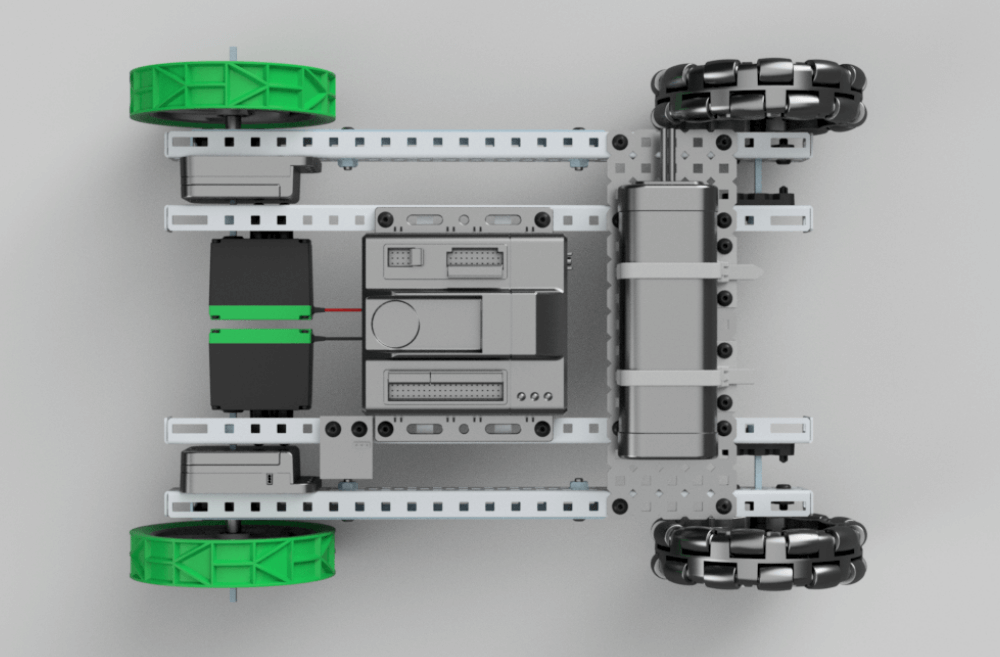
\includegraphics[width=.475\linewidth]{robot2.png}}}%

    \caption{3D Model robota}%
    \label{img:3D Model robota}%
  \end{figure}

  Po úspěšném testování a odladění kódu jsou implementace a jejích odvození v článku jednoduchým způsobem (pokud možno obohacené názornými ilustracemi a vizualizacemi) vysvětleny. Na konci je zpravidla rozebírána použitelnost daných konceptů v reálné robotice a nastíněny navazující články v rámci daného tematického okruhu.


  \subsubsection{Vizualizace} \label{sec:Vizualizace}
  Vizualizace jsou implementovány v jazyce JavaScript s využitím knihovny p5.js (viz. kapitola~\ref{sec:p5.js}). Jsou uzpůsobeny pro ovládání myší či dotykem, aby byly funkční jak na osobních počítačích, tak na mobilech. Offline verze stránky vizualizace neobsahuje, protože formát \gls{pdf} vkládání kódu kvůli bezpečnosti neumožňuje~\cite{history-of-pdf}.


  \subsubsection{Ilustrace} \label{sec:Ilustrace}
  Ke tvorbě ilustrací je používán program na tvorbu vektorové grafiky Inkscape (viz. kapitola~\ref{sec:Inkscape}) v kombinaci s \gls{cad} softwarem Fusion 360 (viz. kapitola~\ref{sec:Fusion 360}).

  Vektorová grafika je pro vytváření ilustrací správná volba z toho důvodu, že potřebné tvary lze vytvářet a upravovat výrazně rychleji a efektivněji než rastr. Zabírá také méně místa a je ukládána v prostém textu, což má oproti binárnímu formátu řadu výhod.

  Příkladem ilustrací článků je obrázek \ref{img:Příklady ilustrací}. Ilustrace pocházejí z článků o odometrii a ilustrují pohyb robota pro výpočet inverzní kinematiky jeho podvozku.

  \begin{figure}[H]
    \centering

    \subcaptionbox{Pohyb robota po kružnici}{\fbox{
\includegraphics[width=.3\linewidth]{illustration1.png}}}%
    \hfill
    \subcaptionbox{Odhad pozice při pohybu po přímce}{\fbox{
\includegraphics[width=.3\linewidth]{illustration2.png}}}%
    \hfill
    \subcaptionbox{Odhad pozice při pohybu po kružnici}{\fbox{
\includegraphics[width=.3\linewidth]{illustration3.png}}}%

    \caption{Příklady ilustrací}%
    \label{img:Příklady ilustrací}%
  \end{figure}


  \subsubsection{Matematika} \label{sec:Matematika}
  Jelikož jsou probírané koncepty a algoritmy založeny na matematice, tak stránka podporuje vkládání rovnic a výrazů do článků. Tuto funkcionalitu zajišťuje JavaScriptová knihovna \KaTeX{} (viz. kapitola~\ref{sec:KaTeX}), díky které lze \LaTeX ové rovnice umísťovat přímo do Markdownových článků.

  Příkladem zápisu matematiky v článku je rovnice~(\ref{eq:katex equation}), která je pomocí \KaTeX u převedena na rovnici~(\ref{eq:converted equation}).

  \begin{equation} \label{eq:katex equation}
    \verb|Je pravda, že $$\sum_{i=1}^{n} i = \frac{n(n+1)}{2}$$.|
  \end{equation}

  \begin{equation} \label{eq:converted equation}
    \text{Je pravda, že }\sum_{i=1}^{n} i = \frac{n(n+1)}{2}\text{.}
  \end{equation}


  \subsection{Struktura}
  Stránka je strukturována do značné míry jako kniha, převážně kvůli plynulosti jejího čtení a zjednodušení jejího převodu do formátu \gls{pdf}.

  Návštěvníka po zobrazení stránky přivítá \emph{úvodní stránka} (obrázek~\ref{img:Úvodní stránka}), která představí projekt a jeho cíle. Příležitostně také obsahuje důležitá sdělení o provozu stránky. Poté následuje \emph{předmluva} (obrázek~\ref{img:Předmluva}), ve které je kromě diskuze o předpokladech pro čtení zodpovězena řada otázek, které by čtenáři mohli při čtení stránky mít.

  \begin{figure}[H]
    \minipage{0.475\textwidth}
      \fbox{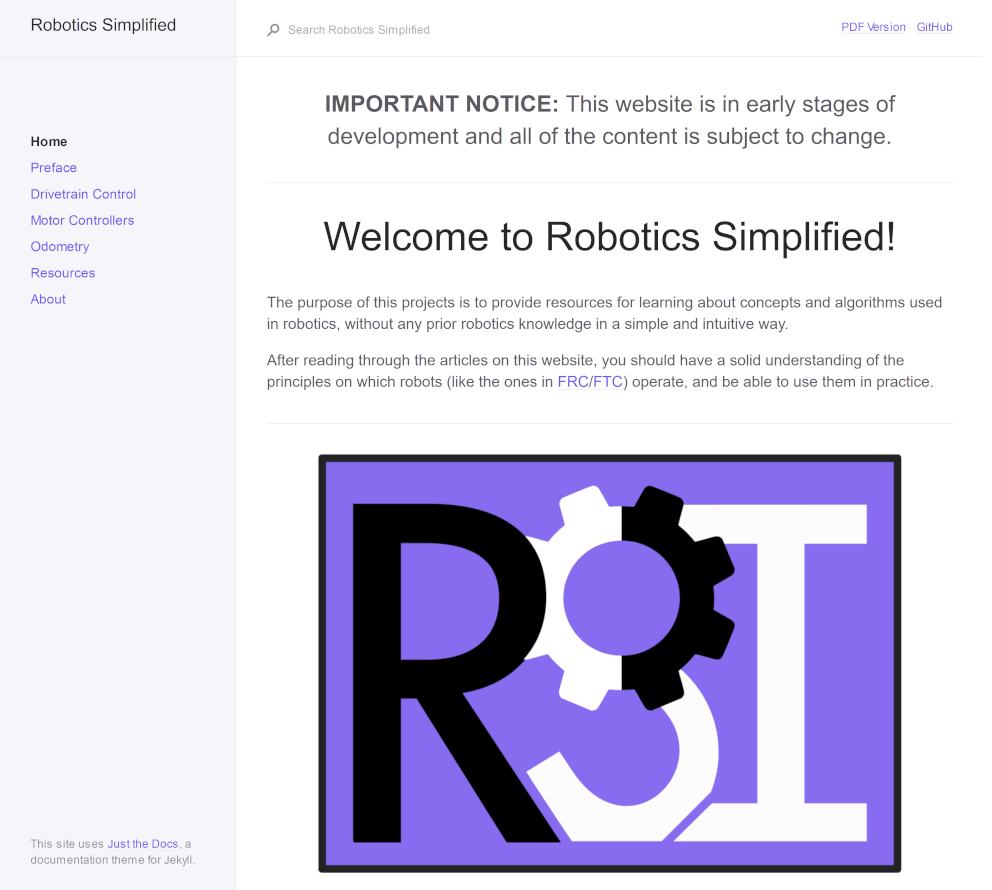
\includegraphics[width=\linewidth]{1.png}}
      \caption{Úvodní stránka} \label{img:Úvodní stránka}
    \endminipage\hfill
     \minipage{0.475\textwidth}
      \fbox{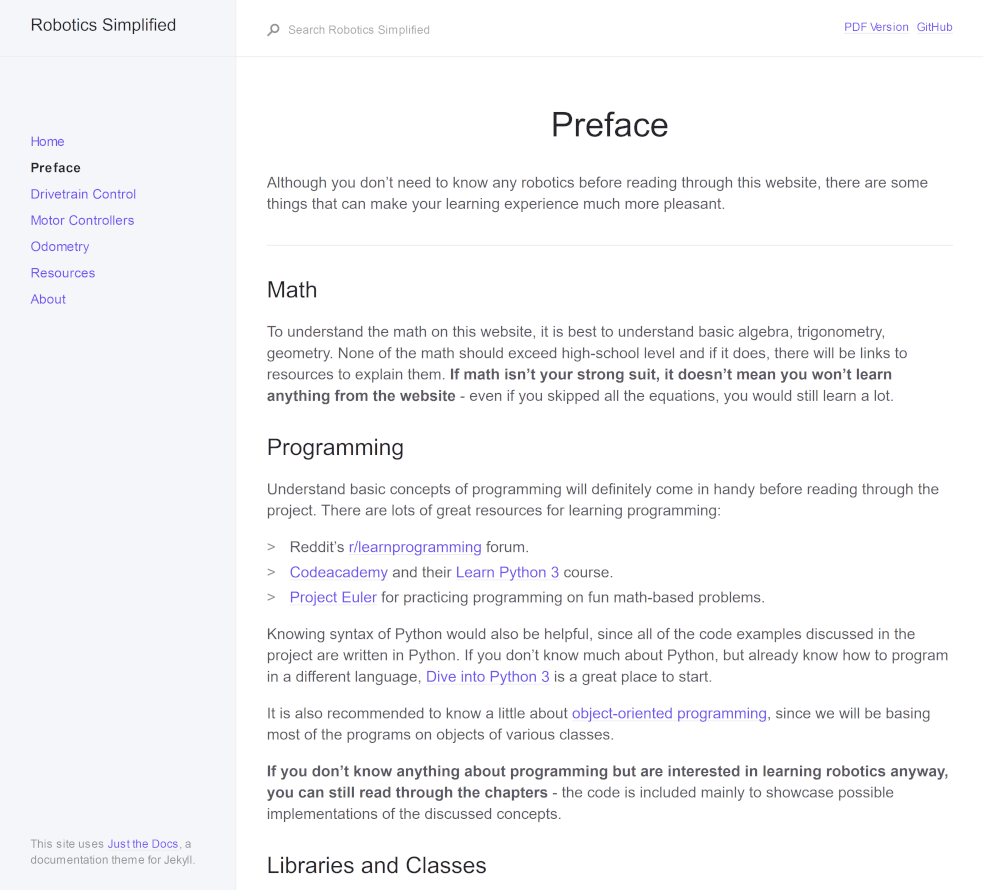
\includegraphics[width=\linewidth]{2.png}}
      \caption{Předmluva} \label{img:Předmluva}
    \endminipage
  \end{figure}

  Hlavní náplní projektu jsou \emph{tematické okruhy} (obrázek~\ref{img:Příklady článků}), které se skládají z článků probírajících koncepty s podobnou tematikou, v pořadí, ve kterém by pro návaznost měly být čteny.

  \begin{figure}[H]
    \centering

    \subcaptionbox{Úvod do ovládání podvozku}{\fbox{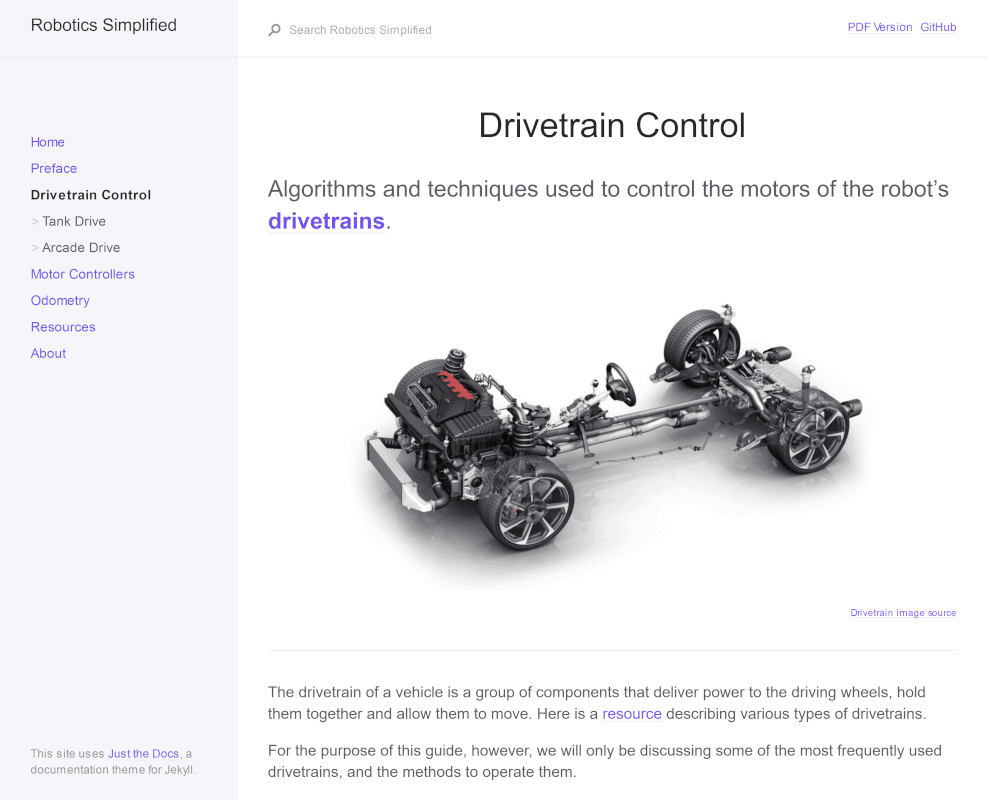
\includegraphics[width=.3\linewidth]{3-1.png}}}%
    \hfill
    \subcaptionbox{Metoda Tank drive pro ovládání podvozku robota}{\fbox{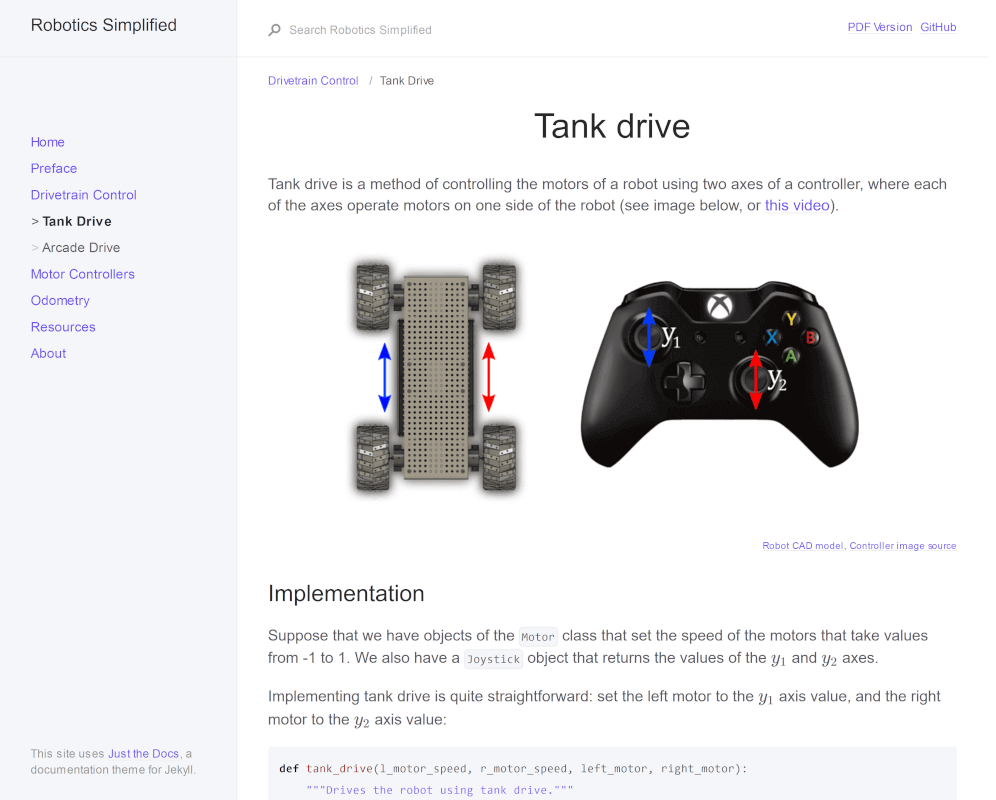
\includegraphics[width=.3\linewidth]{3-2.png}}}%
    \hfill
    \subcaptionbox{Výpočet úhlu z enkóderů}{\fbox{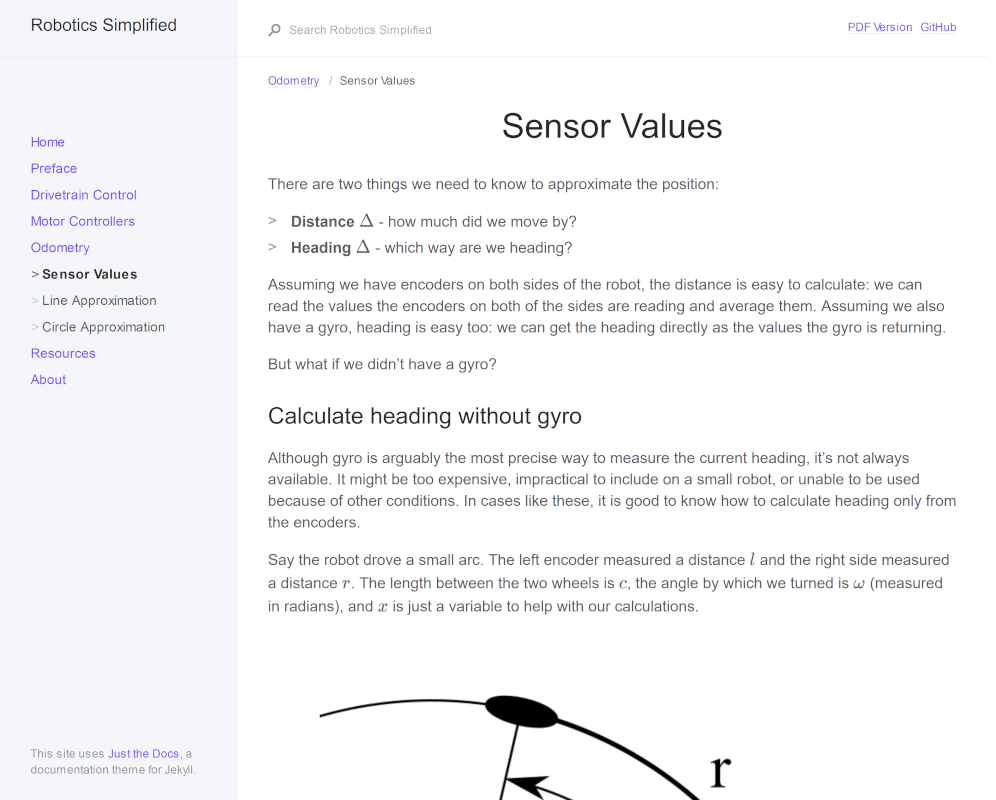
\includegraphics[width=.3\linewidth]{3-3.png}}}%

    \caption{Příklady článků}%
    \label{img:Příklady článků}%
  \end{figure}

  Na závěr je přiložen článek s \emph{dodatečnými materiály} (obrázek~\ref{img:Dodatečné materiály}) použitými při tvorbě projektu a sekce \emph{O nás} (obrázek~\ref{img:O nás}), která popisuje důvod za vznikem projektu, návod na případnou spolupráci na projektu a poděkování.

  \begin{figure}[H]
    \minipage{0.475\textwidth}
      \fbox{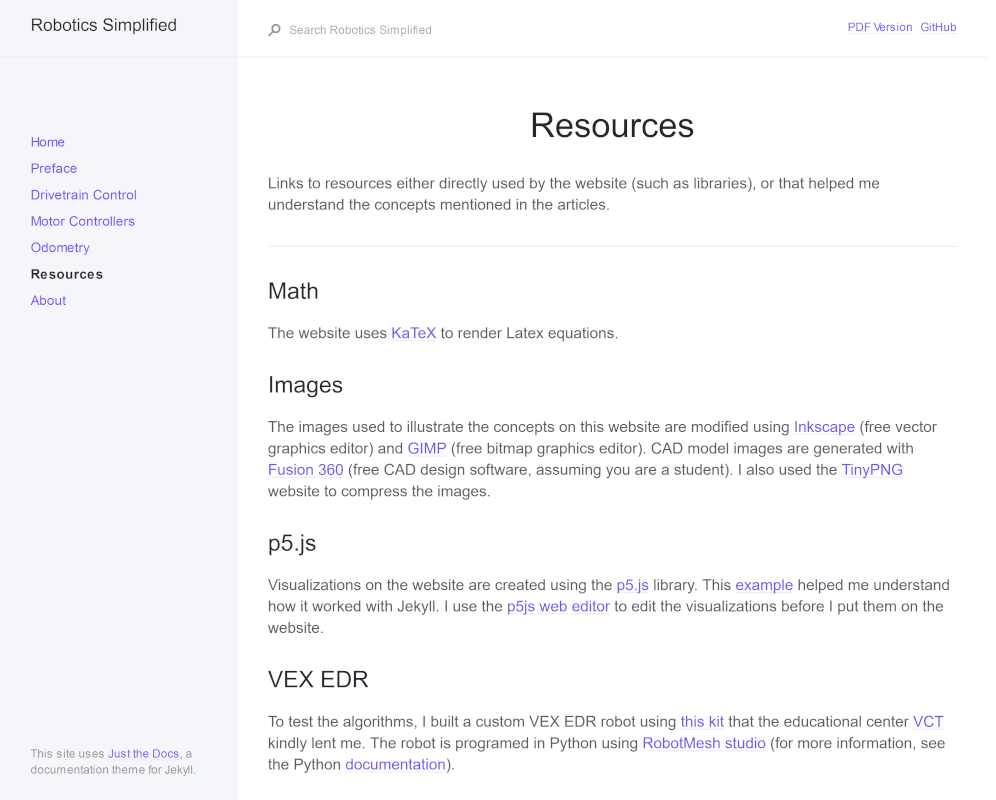
\includegraphics[width=\linewidth]{4.png}}
      \caption{Dodatečné materiály} \label{img:Dodatečné materiály}
    \endminipage\hfill
     \minipage{0.475\textwidth}
      \fbox{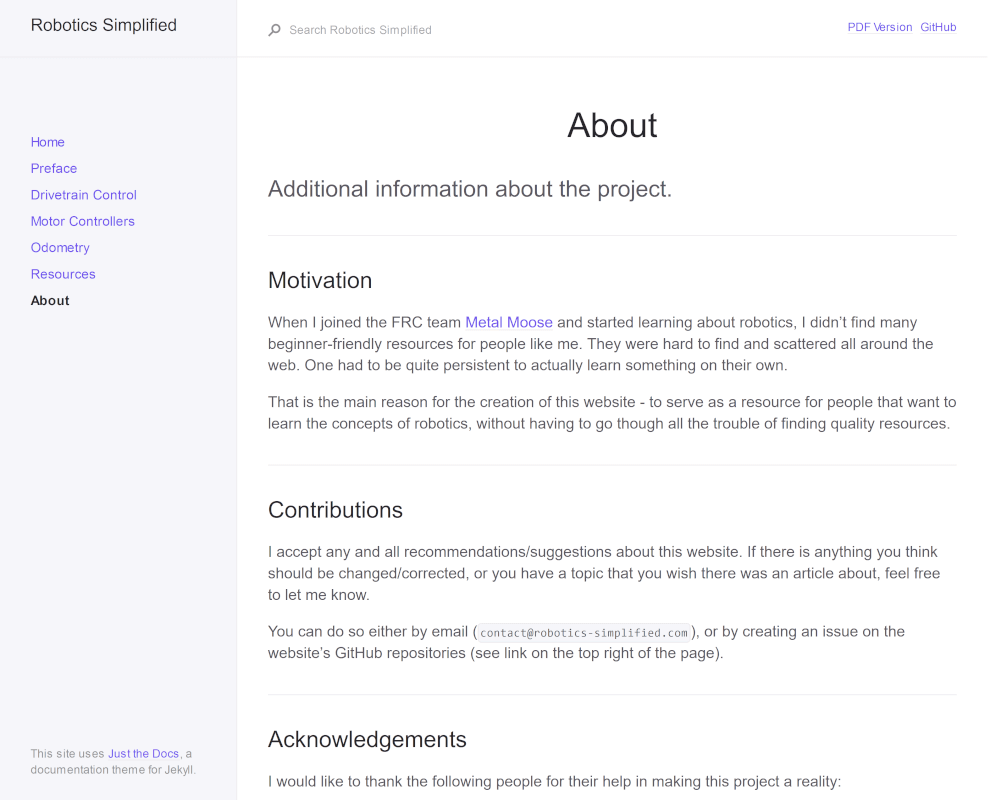
\includegraphics[width=\linewidth]{5.png}}
      \caption{O nás} \label{img:O nás}
    \endminipage
  \end{figure}


  \subsection{Uplatnění}
  Kromě snahy o zpřístupnění robotiky pro začátečníky stránka rovněž poskytuje zdroj strukturovaných vzdělávacích materiálů pro lektory kurzů robotiky a programování. Sám jich několik na Vzdělávacím centru Turnov pomocí mé stránky vyučuji a mé zkušenosti byly zatím pouze kladné.

  Díky otevřenosti zdrojového kódu stránka dále slouží jako šablona pro Jekyllem poháněné projekty, které by rády docílily obdobné funkcionality (rovnice, automatizace pomocí skriptů, zvýrazňování syntaxe kódu, aj.) bez zdlouhavého psaní a ladění kódu.


  \section{Automatizace provozu stránky} \label{sec:Automatizace provozu stránky}
  Ke tvorbě kvalitního vzdělávacího materiálu je potřeba plynulý a do nejvyšší možné míry automatizovaný provoz stránky~--~k přidání nového článků by mělo stačit v příslušné složce projektu vytvořit nový soubor a zbytek procesu by měl proběhnout bez zásahu autora.

  Stránka je v tomto duchu automatizována skripty psanými v jazyce Python (viz. kapitola~\ref{sec:Python}), aby se autor mohl plně soustředit na práci.


  \subsection{Nahrání obsahu přes \acrshort{ftp}}
  \gls{ftp} je protokol zprostředkovávající přenos souborů mezi počítači po síti. Od prvního návrhu pro využití na \gls{mit} v roce 1971 až po oficiální specifikaci publikovanou roku 1985 prošel mnoha revizemi, s dodatky přidávanými dodnes~\cite{ftp-specification}. Jedná se o populární volbu protokolu pro hostingy webových stránek a hosting tohoto projektu není výjimkou.

  Script \texttt{upload.py} se po zadání hesla připojí přes protokol \gls{ftp} na server, rekurzivně smaže soubory a adresáře aktuální verze stránky a nahraje verzi novou. Pro dodatečné zabezpečení je \gls{ip} serveru šifrována symetrickou šifrou \gls{aes}.


  \subsection{Generování souboru sitemap.xml}
  Soubor protokolu sitemap obsahuje informace o pořadí procházení, časech změny a relativních prioritách částí stránky. Je využíván vyhledávacími portály, které soubory tohoto typu využívají pro efektivnější indexování stránky ve svém systému.

  Script \texttt{sitemap.py} podle pořadí článků generuje záznamy do souboru \texttt{sitemap.xml}. Informace o umístění a poslední úpravě jsou získávány z atributů souborů a priorita je přidělena podle jejich pozice na stránce~--~úvodní stránka má prioritu $1.0$, hlavní články mají prioritu $0.8$ a vedlejší články prioritu $0.6$.


  \subsection{Převod webové stránky do \acrshort{pdf}} \label{sec:Převod webové stránky do PDF}
  Pro offline dostupnost existuje mnoho různých typů souborů, na které by stránka šla převést. Často používané formáty jako \gls{doc} a \gls{docx} jsou však pro použití v projektu nevhodné, protože se mohou na různých zařízeních zobrazit rozdílně. Je tedy vhodnější použít formáty jako \gls{ps} či \gls{pdf}, jejichž vizáž na prostředí závislá není~\cite{history-of-pdf}.

  Přímočará varianta by byla převést články do \gls{pdf} libovolným programem pro převod textových formátů (jako Pandoc). Tímto přístupem by však bylo obtížné generovat obsah a prakticky nemožné ovlivnit výsledné formátování, což potřebám projektu nevyhovuje.

  Pro potřeby projektu byl tedy zvolen převod článků do formátu \LaTeX{} (viz. kapitola~\ref{sec:TeX}) a až poté do \gls{pdf}, což všechny nevýhody první varianty elegantně řeší.

  Script \texttt{tex.py} získá pořadí článků, spojí je za sebe do jednoho dokumentu a poté na ně aplikuje řadu regulárních výrazů, které provedou převod z formátu Markdown do formátu \LaTeX.


  \subsection{Komprimace obrázků}
  Komprimaci obrázků stránky pro zmenšení její velikosti provádí skript \texttt{compress.py}, který pomocí služby TinyPNG a jejího Python \gls{api} všechny obrázky zkomprimuje. Samotný \gls{api} klíč je pro zamezení zneužití šifrován symetrickou šifrou \gls{aes}.

  Úprava fotek funguje na principu \emph{kvantování barev}~--~podobné barvy jsou spojeny do jedné, čímž lze z tradičních 24-bitových palet \gls{png} udělat palety 8-bitové a zmenšit tím obrázek bez výrazného zhoršení kvality.

  Ke 24. únoru 2019 tento skript zkomprimuje obrázky webové stránky na $72.3$ \% jejich původní velikosti a zmenší tím jejich velikost o \emph{262 KB}.


  \subsection{Minimalizace zdrojového kódu}
  Zkompaktnění zdrojového kódu je další možná optimalizace, kterou lze načítání stránky urychlit. Prohlížečům na vzhledu kódu nezáleží a běžné uživatele nezajímá, proto jej lze na úkor čitelnosti zmenšit.

  Tuto funkci zastává skript \texttt{minify.py}, který soubory typu \gls{css} a \gls{html} zmenší odstraněním komentářů, nepotřebných tagů a uvozovek, přebytečných mezer a dalších částí kódu, které po jejich odstranění funkcionalitu kódu nezmění.

  Ke 24. únoru 2019 tento skript zkompaktní \gls{css} a \gls{html} webové stránky na $72.89$ \% a $68.12$ \% jejich původní velikosti a zmenší tím jejich velikost o \emph{129 KB}.


  \subsection{Automatizace procesu}
  Po přidání či úpravě článku je potřeba verzi stránky na hostingu aktualizovat. Tento proces řídí skript \texttt{deploy.py}, který stránku nejprve pomocí Jekyllu vygeneruje, poté ve správném pořadí spustí všechny skripty pro generování dodatečného obsahu a optimalizace a nakonec i skript pro nahrání stránky na webhosting.


  \section{Návštěvnost a zpětná vazba stránky}
  Po publikování webové stránky je pro měření její úspěšnosti třeba sbírat informace o její návštěvnosti a ohlase jejich návštěvníků. Podle těch lze následně uzpůsobit její obsah a vzhled, a zlepšit tím jak kvalitu, tak návštěvnost.

  Následující kapitola rozebírá metody získávání a opodstatňuje hodnoty sbíraných dat. Rovněž také popisuje metody k obdržení zpětné vazby o webové stránce a uvádí její příklady.


  \subsection{Analýza návštěvnosti}
  Google je jedna z nejúspěšnějších technologicky zaměřených společností dneška. Specializuje se na reklamní technologie, internetové vyhledávání a řadu dalších technických oborů. V projektu jsou služby této společnosti používany především kvůli jednoduchosti jejich konfigurace a popularitě webového vyhledávače Google.

  \emph{Google Analytics} slouží k analýze návštěvnosti webových stránek. Pro použití stačí na danou stránku přidat JavaScriptovou knihovnu, která shromažďuje informace o návštěvnících (z údajů prohlížeče a také \gls{http} cookies) a jejich interakcí s danou webovou stránkou.

  Kromě služby Google Analytics je dále používána služba \emph{Google Search Console}, která zobrazuje statistiky o indexování webové stránky v rámci vyhledávání Google~--~její průměrné pozice při relevantních vyhledáváních, počet zobrazení, indexované podstránky, aj. Kromě toho informuje správce stránky o potenciálních problémech jako špatném zobrazením na mobilních zařízeních či chybně vygenerovaném souboru \texttt{sitemap.xml}.

  Celková návštěvnost stránky v období od 18. prosince 2018 (počátek měření) k 18. březnu 2018 činí \emph{466} návštěvníků. Jejich demografické údaje zachycují grafy \fullref{img:Pohlaví návštěvníků stránky} a \fullref{img:Věk návštěvníků stránky}.

  \begin{minipage}[b]{0.475\textwidth}
    \footnotesize
    \centering
    \begin{tikzpicture}
      \pie[color={blue!70, red!70}, rotate=-35, before number=\ScanPercentage, after  number ={ }\%,]{91.2/Muži, 8.8/Ženy}
    \end{tikzpicture}
    \captionof{figure}{Pohlaví návštěvníků stránky}
    \label{img:Pohlaví návštěvníků stránky}
  \end{minipage}\hfill
  \begin{minipage}[b]{0.475\textwidth}
    \footnotesize
    \centering
    \begin{tikzpicture}
      \begin{axis}[
        symbolic x coords={18--24, 25--34, 35--44, 45--54},
        xtick=data,
        ylabel={Procento návštěvníků},
        xlabel={Věková kategorie},
        bar width=1cm,
        width=\textwidth,
        enlarge x limits=0.18,
        ymin=0, ymax=60,
        nodes near coords={\pgfmathprintnumber\pgfplotspointmeta{ }\%},
        yticklabel={\pgfmathparse{\tick}\pgfmathprintnumber{\pgfmathresult}{ }\%},]
        \addplot[ybar,fill=blue] coordinates {
          (18--24, 18.9)
          (25--34, 48.4)
          (35--44, 18.0)
          (45--54, 14.7)
        };
      \end{axis}
    \end{tikzpicture}
    \captionof{figure}{Věk návštěvníků stránky}
    \label{img:Věk návštěvníků stránky}
  \end{minipage}

  Údaje o přístupu ke stránce jsou dále zaneseny do tabulek \fullref{tab:Návštěvnost stránky podle země} a \fullref{tab:Návštěvnost stránky podle prohlížeče}.

  \vspace{-0.5\parskip}
  \begin{minipage}[b]{0.475\textwidth}
    \begin{table}[H]
      \caption{Návštěvnost stránky podle země}
      \label{tab:Návštěvnost stránky podle země}
      \footnotesize
      \centering
      \ra{1.3}
      \begin{tabular}{*5l}
        \toprule
        \emph{Země} & \emph{Počet návštěvníků} \\
        \midrule
        Spojené státy americké & 240 \\
        Česká republika	       & 35 \\
        Spojené království     & 20 \\
        Kanada                 & 17 \\
        Německo                & 10 \\
        Japonsko               & 10 \\
        Čína                   & 8 \\
        Indie                  & 8 \\
        Španělsko              & 7 \\
        Nizozemí               & 7 \\
        \bottomrule
      \end{tabular}
    \end{table}
  \end{minipage}\hfill
  \begin{minipage}[b]{0.475\textwidth}
    \begin{table}[H]
      \caption{Návštěvnost stránky podle prohlížeče}
      \label{tab:Návštěvnost stránky podle prohlížeče}
      \footnotesize
      \centering
      \ra{1.3}
      \begin{tabular}{*5l}
        \toprule
        \emph{Prohlížeč} & \emph{Počet návštěvníků} \\
        \midrule
        Chrome            & 226 \\
        Firefox	          & 111 \\
        Safari            & 85 \\
        Android Webview   & 14 \\
        Internet Explorer & 6 \\
        Opera             & 6 \\
        Edge              & 5 \\
        Samsung Internet  & 5 \\
        Neurčeno          & 4 \\
        Cốc Cốc           & 1 \\
        \bottomrule
      \end{tabular}
    \end{table}
  \end{minipage}

  % TODO: write something about the results


  \subsection{Získávání zpětné vazby}
  K získání zpětné vazby o technicky zaměřeném projektu je vhodné použít webové stránky s obdobnou tématikou. Projekt byl z tohoto důvodů zveřejněn na následujících internetových fórech:

  {\parskip=0pt
  \begin{itemize}[topsep=\itemsep]
    \item \emph{ChiefDelphi}~--~internetové fórum zaměřené na soutěž \gls{frc}, převážně pro členy \gls{frc} týmů.
    \item \emph{Reddit}~--~jedno z nejpopulárnějších internetových fór dneška. Zajímavostí jsou subreddity~--~samospravované celky, na kterých jsou zveřejňovány články se společnou tématikou.
    \begin{itemize}[topsep=0pt]
      \item \emph{Subreddit \gls{frc}}~--~zaměření na soutěž \gls{frc}, od vtipných obrázků a videí po odborné články. Časté jsou též novinky a události ze světa soutěže.
      \item \emph{Subreddit Robotics}~--~většina příspěvků jsou vzdělávacího charakteru. Časté druhy příspěvků jsou videa a články o domácích projektech uživatelů tohoto fóra.
    \end{itemize}
    \item \emph{Hacker News}~--~internetové fórum, které je ve svém fungování blízké Redditu. Není však dále strukturováno na subreddity a obsah je vážnějšího charakteru~--~světové novinky, nové výzkumy a odborné práce, měsíční přehledy dostupných pracovních pozic \gls{it} firem, apod.
  \end{itemize}}

  Zpětná vazba obsahovala rady na potenciální možnost zpeněžení webové stránky přidáním reklam, zlepšení kompatibility s obskurnějšími nastaveními prohlížečů a umožnění upravovat samotné ukázky kódu a měnit tím chování vizualizace.

  \newpage

  \section{Závěr}
  % TODO: sum-up the results of the paper

  Náplní práce na projektu je v dohledné budoucnosti tvorba nových článků a jejich lokalizace do českého jazyka. S tím je též úzce spjata revize již napsaných článků~--~přidávání dodatečných ilustrací a vizualizací, zpřehlednění textu, revize kódu, aj.

  Stránka rovněž nepoužívá protokol \gls{https}, který na rozdíl od \gls{http} šifruje komunikaci mezi klientem a serverem a zamezuje tím řadě možných útoků, před kterými \gls{http} uživatele nechrání. Jelikož však WEDOS podporuje mezinárodně uznávanou certifikační autoritu Let's Encrypt, tak by tato změna příliš komplikovaná být neměla.

  Další oblastí zlepšení je převod webové stránky do offline verze~--~export do formátů jako \gls{epub} a \gls{mobi} pro zlepšení podpory elektronických čteček knih, zajištění větší spolehlivosti převodu a implementace dodatečných funkcí (přeškrtnutí textu, podtržení textu, reference, citace...).

  % TODO: compare other works

  \newpage

  % create the bibliography
  \printbibliography[heading=bibnumbered, title=Použitá literatura]

  \newpage

  % create lof and lot
  \section{Seznam obrázků a tabulek}
  {%
  \let\oldnumberline\numberline%
  \renewcommand{\numberline}{\figurename~\oldnumberline}%
  \listoffigures%
  }
  \vspace{\baselineskip}
  {%
  \let\oldnumberline\numberline%
  \renewcommand{\numberline}{\tablename~\oldnumberline}%
  \listoftables%
  }

  \newpage

  \section{Příloha 1: Zdrojový kód stránky} \label{sec:Příloha 1: Zdrojový kód webové stránky}

  \newpage

  \section{Příloha 2: Data testování doby načtení} \label{sec:Příloha 2: Data testování doby načtení}
  Tabulka \ref{tab:Data testování doby načtení} obsahuje místa, ze kterých byla testována doba načtení stránky \url{http://robotics-simplified.com/} a částečné odkazy na testovací data. K vytvoření úplného odkazu stačí před označení daného města přidat \texttt{www.webpagetest.org/result/}.

  \begin{table}[H]
    \caption{Data testování doby načtení}
    \label{tab:Data testování doby načtení}
    \footnotesize
    \centering
    \ra{1.3}
    \begin{tabular}{*5l}
      \toprule
      \emph{Lokace}            & \emph{Označení}                      \\ \midrule
      Argentina (Buenos Aires)        & \href{https://www.webpagetest.org/result/190213_PC_5d05753a2ce2126089db6b8726171c13}{\texttt{190213\_PC\_5d05753a2ce2126089db6b8726171c13}} \\
      Austrálie (Sydney)              & \href{https://www.webpagetest.org/result/190213_8N_c4802d60f2820dd2b7f8e3e5d6a384c1}{\texttt{190213\_8N\_c4802d60f2820dd2b7f8e3e5d6a384c1}} \\
      Belgie (Brusel)                 & \href{https://www.webpagetest.org/result/190213_PK_8973798f51f040a199501b3332071bc2}{\texttt{190213\_PK\_8973798f51f040a199501b3332071bc2}} \\
      Brazílie (Sao Paulo)            & \href{https://www.webpagetest.org/result/190213_AD_d2d6ea6b39f36853cf476a5f1d1f3092}{\texttt{190213\_AD\_d2d6ea6b39f36853cf476a5f1d1f3092}} \\
      Česká republika (Praha)         & \href{https://www.webpagetest.org/result/190213_SD_119a43e321c4360178004f09bb4d27a0}{\texttt{190213\_SD\_119a43e321c4360178004f09bb4d27a0}} \\
      Čína (Hong Kong)                & \href{https://www.webpagetest.org/result/190213_NK_dfd8ddf4b9766b3386799de124a67ad8}{\texttt{190213\_NK\_dfd8ddf4b9766b3386799de124a67ad8}} \\
      Francie (Strasburg)             & \href{https://www.webpagetest.org/result/190213_35_5db33eb4e90d8b096d8853fa453d54d3}{\texttt{190213\_35\_5db33eb4e90d8b096d8853fa453d54d3}} \\
      Indie (Mumbai)                  & \href{https://www.webpagetest.org/result/190213_ED_2a0542955442372c423c9306a7492c02}{\texttt{190213\_ED\_2a0542955442372c423c9306a7492c02}} \\
      Indonésie (Jakarta)             & \href{https://www.webpagetest.org/result/190213_12_db0913a1b2708f54db46d5d40b7f61e5}{\texttt{190213\_12\_db0913a1b2708f54db46d5d40b7f61e5}} \\
      Itálie (Milán)                  & \href{https://www.webpagetest.org/result/190213_QE_7d2d0c62fe56d0a992f83872fea9589a}{\texttt{190213\_QE\_7d2d0c62fe56d0a992f83872fea9589a}} \\
      Izrael (neurčeno)               & \href{https://www.webpagetest.org/result/190213_XT_735a3f35ee6a8056ad47aac3d5a95917}{\texttt{190213\_XT\_735a3f35ee6a8056ad47aac3d5a95917}} \\
      Japonsko (Tokio)                & \href{https://www.webpagetest.org/result/190213_8Q_083b45677c2c51f4fe7bd25b554dff38}{\texttt{190213\_8Q\_083b45677c2c51f4fe7bd25b554dff38}} \\
      Jižní Korea (Soul)              & \href{https://www.webpagetest.org/result/190213_TX_d56f64b9948b96bdfdd1323fd16b0867}{\texttt{190213\_TX\_d56f64b9948b96bdfdd1323fd16b0867}} \\
      Kanada (Toronto)                & \href{https://www.webpagetest.org/result/190213_44_a861d3caa2bdbb547775b76e0ca7e357}{\texttt{190213\_44\_a861d3caa2bdbb547775b76e0ca7e357}} \\
      Nizozemí (Amsterdam)            & \href{https://www.webpagetest.org/result/190213_37_88f29978d6231e700fe963b8d943a79b}{\texttt{190213\_37\_88f29978d6231e700fe963b8d943a79b}} \\
      Německo (Berlín)                & \href{https://www.webpagetest.org/result/190213_S3_321db7231844fc993d91fba974e569bb}{\texttt{190213\_S3\_321db7231844fc993d91fba974e569bb}} \\
      Polsko (Varšava)                & \href{https://www.webpagetest.org/result/190213_AV_e12420619d2b67b02b36fd8f85012634}{\texttt{190213\_AV\_e12420619d2b67b02b36fd8f85012634}} \\
      Spojené arabské emiráty (Dubaj) & \href{https://www.webpagetest.org/result/190213_66_d158a4ae09a1ef5d63b68693b5230066}{\texttt{190213\_66\_d158a4ae09a1ef5d63b68693b5230066}} \\
      Spojené království (Londýn)     & \href{https://www.webpagetest.org/result/190213_SS_1226a99822746d3cf16fb81bd19c9ac8}{\texttt{190213\_SS\_1226a99822746d3cf16fb81bd19c9ac8}} \\
      Spojené státy americké (Clifton)& \href{https://www.webpagetest.org/result/190213_3S_570bc4b76dd084486a1ae6ba1829f2cc}{\texttt{190213\_3S\_570bc4b76dd084486a1ae6ba1829f2cc}} \\
      Španělsko (La Rioja)            & \href{https://www.webpagetest.org/result/190213_ZA_96b8ca66a5af8d0bbee48a48d1ebf901}{\texttt{190213\_ZA\_96b8ca66a5af8d0bbee48a48d1ebf901}} \\
      Švédsko (Stockholm)             & \href{https://www.webpagetest.org/result/190213_PC_8bf596590b3cb93164fb6b20e2ae9b7a}{\texttt{190213\_PC\_8bf596590b3cb93164fb6b20e2ae9b7a}} \\
      Turecko (Istanbul)              & \href{https://www.webpagetest.org/result/190213_FZ_3eb94a70dfdd8c92bcfcfaf74a412501}{\texttt{190213\_FZ\_3eb94a70dfdd8c92bcfcfaf74a412501}} \\
      Vietnam (neurčeno)              & \href{https://www.webpagetest.org/result/190213_RQ_18f2a02931599884f8922a3ce09f56bc}{\texttt{190213\_RQ\_18f2a02931599884f8922a3ce09f56bc}} \\
      \bottomrule
    \end{tabular}
  \end{table}

  \newpage

  \section{Příloha 3: \acrshort{step} model robota} \label{sec:STEP model robota}
\end{document}
